\documentclass[10pt]{beamer}
\usepackage{mathrsfs}


\usepackage[T2A]{fontenc}
\usepackage[utf8]{inputenc}
\usepackage[russian,english]{babel}

\usefonttheme[onlymath]{serif}

\usetheme[progressbar=frametitle]{metropolis}
\usepackage{appendixnumberbeamer}

\usepackage{booktabs}
\usepackage[scale=2]{ccicons}

\usepackage{pgfplots}
\usepgfplotslibrary{dateplot}

\usepackage{xspace}
\newcommand{\themename}{\textbf{\textsc{metropolis}}\xspace}
\newcommand{\TODO}[1]{\textbf{\textcolor{red}{TODO: #1}}}

\date{}
\author{Екатерина Тузова}


\title{Лекция 12}
\subtitle{Методы восстановления регрессии}

\begin{document}

\section{Разбор летучки}

\maketitle

\begin{frame}\frametitle{Регрессия}
	$X$-- объекты в $\mathbb{R}^n$; Y — ответы в $\mathbb{R}$\\
	$X^l = (x_i, y_i)_{i=1}^l$ -- обучающая выборка\\
	$y_i = y(x_i)$,  $y : X \rightarrow Y$ -- неизвестная зависимость\\
	\bigbreak
	$a(x) = f (x, w)$ -- модель зависимости,\\
	$w \in \mathbb{R}^p$ -- вектор параметров модели.\\
	\bigbreak
	Метод наименьших квадратов (МНК):\\
	$$Q(w,X^l) = \sum\limits_{i=1}^l \alpha_i (f (x_i, w) - y_i)^2 \rightarrow \min\limits_{w}$$\\
\end{frame}

\section{К ближайших соседей}

\begin{frame}{К ближайших соседей}
  ${\rho(u, x_1) \leq \rho(u, x_2) \leq \dots \leq \rho(u, x_l)}$\\
  \bigbreak
	${x_i}$ -- $i$-й сосед объекта $u$\\
	${y_i}$ -- класс $i$-го соседа $u$
  \bigbreak
  \alert{Идея 1}: Посмотрим на ближайшие объекты и отнесем $u$ к доминирующему классу. 
  \bigbreak
  \pause
  \alert{Идея 2}: Более близкие объекты важнее для классификации.
\end{frame}

\begin{frame}{К ближайших соседей}
  $a(u, X^l) = \arg\max\limits_{y \in Y} \sum\limits_{y_i = y} w(i, u)$\\
  \bigbreak
  ${w(i, u) = [i \leq k]}$
\end{frame}

\section{Как использовать для задачи регрессии?}

\begin{frame}{K neighbors regressor}
  \alert{Идея}: Усреднить характеристики $k$ ближайших соседей.\\
  \pause
  \bigbreak
  $a(u, X^l) = \frac{1}{k} \sum\limits_{i=1}^k w(i, u)*y_i$
\end{frame}

\begin{frame}{Пример}
  \centering
  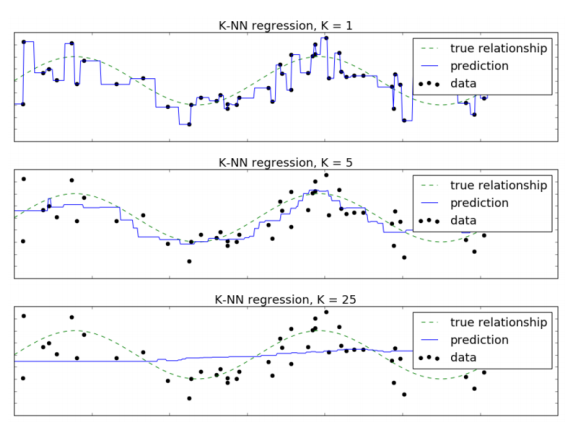
\includegraphics[width=0.9 \textwidth, keepaspectratio]{images/knn}
\end{frame}

\section{Деревья принятия решений}

\begin{frame}{Бинарное решающее дерево}
	Бинарное решающее дерево -- алгоритм классификации $a(x, \beta)$, задающийся бинарным деревом:\\
	\begin{enumerate}[--]
  	  \item $\forall v \in V_{inner} \rightarrow \beta_v: X \rightarrow \left\{ 0,1\right\}$, $\beta \in \mathscr{B}$
	  \item $\forall v \in V_{leaf} \rightarrow $ имя класса $c_v \in Y$\\
	\end{enumerate}	

	\begin{figure}[htbp]
	  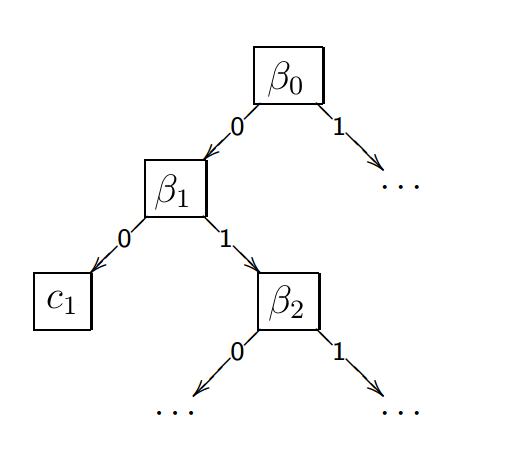
\includegraphics[height=150pt, keepaspectratio = true]{images/binary_tree}   
	\end{figure}
\end{frame}

{\foot{Iterative Dichotomizer 3}
\begin{frame}{Алгоритм построения ID3}
  \begin{algorithmic}[1]
    \Function{LearnID3}{$U$, $\mathscr{B}$}
       \If {все объекты из $U$ лежат в одном классе $c \in Y$}
         \State \Return {новый лист $v$, $c_v = c$}
       \EndIf
       \State $\beta^* = \max\limits_{\beta \in \mathscr{B}} I(\beta, U)$
       \State $U_{left} = \left\{ x \in U : \beta^*(x) = 0\right\}$	
       \State $U_{right} = \left\{ x \in U : \beta^*(x) = 1\right\}$	
       \If {$U_{left} = \oslash$ или $U_{right} = \oslash$}
         \State \Return {$v$, $c_v$ = Majority($U$)}
       \EndIf
       \State Создать новую внутреннюю вершину $v$: $\beta_v = \beta^*$
       \State $L_v =$ LearnID3 ($U_{left}$, $\mathscr{B}$)
       \State $R_v =$ LearnID3 ($U_{right}$, $\mathscr{B}$)
       \State \Return $v$
    \EndFunction
  \end{algorithmic}    
\end{frame}
}

\section{Как использовать для задачи регрессии?}

\begin{frame}{Decision tree regression}
  \alert{Идея}: В каждый узел дерева записать среднее значение целевой функции. 
  \pause
  \bigbreak
  \alert{Идея}: Используется критерий Джини. Хотим, чтобы выборка разбивалась таким образом, что значения целевого признака в каждом листе примерно равны.
  \pause
  \bigbreak
  $$I(\beta,X^l)= \sum\limits_{i=1}^n y_i(1 - y_i)$$
  $n$ -- количество объектов в листе
\end{frame}

\begin{frame}{Пример}
  \centering
  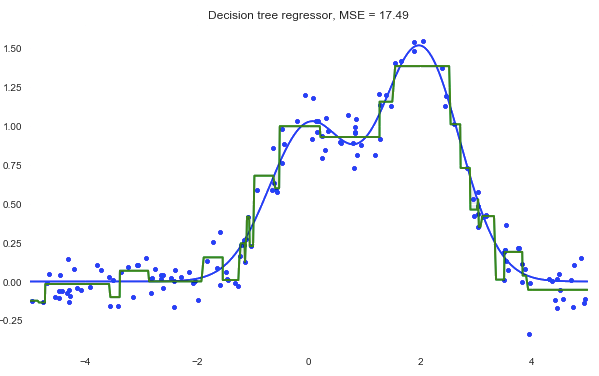
\includegraphics[width=0.9 \textwidth, keepaspectratio]{images/decision_tree}
\end{frame}

\section{Нейронные сети}

\begin{frame}{Многослойная нейронная сеть}
	Пусть $Y = \mathbb{R}^M$, два слоя в сети.\\
	
	\begin{figure}[htbp]
	  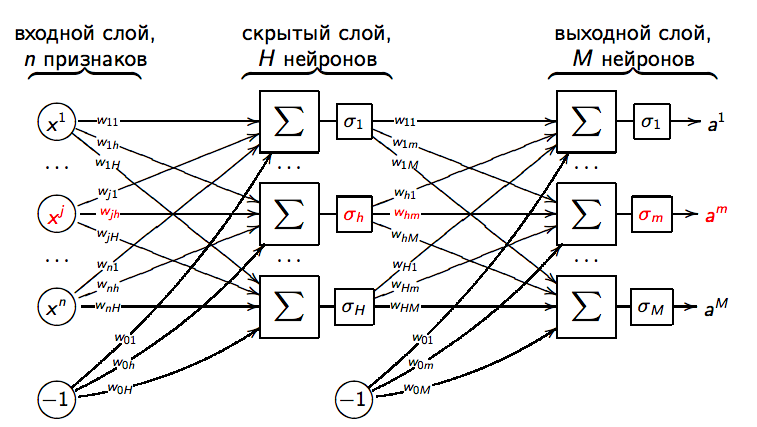
\includegraphics[height=150pt, keepaspectratio = true]{images/neural_network}   
	\end{figure}
\end{frame}

{\foot{Backpropagation}
\begin{frame}{Алгоритм обратного распространения ошибки}
  \begin{algorithmic}[1]
    \Function{Backpropagation}{$X^l$, $H$, $\alpha$, $\eta$}
     \State \dots
     \MRepeat [пока $Q$ не стабилизируются] 
       \State Взять $x_i$ из $X^l$
       \pause
       \State 	$\begin{cases}
	\hspace{5mm} u^h_i = \sigma_h (\sum\limits_{j=0}^J w_{jh} x_i^j), \hspace{4mm} h = 1, \dots, H\\
	\hspace{5mm} a^m_i = \sigma_m (\sum\limits_{h=0}^H w_{hm} u_i^h), \hspace{4mm} \varepsilon_i^m = a_i^m - y_i^m, \hspace{4mm} m = 1, \dots, M\\
	\hspace{5mm} \mathcal{L}_i = \frac{1}{2} \sum\limits_{m=1}^M (\varepsilon_i^m)^2\\
	\end{cases}$\\
	\pause
	$\begin{cases} \hspace{5mm} \varepsilon_i^h = \sum\limits_{m=1}^M \varepsilon_i^m \sigma'_m w_{hm}, \hspace{4mm} h = 1, \dots, H\end{cases}$\\
	\pause
	$\begin{cases} \hspace{5mm} w_{hm} = w_{hm} - \alpha \varepsilon_i^m \sigma'_m u_i^h, \hspace{4mm} h = 0, \dots, H, \hspace{4mm} m = 1, \dots, M\\
	\hspace{5mm} w_{jh} = w_{jh} - \alpha \varepsilon_i^h \sigma'_h x_i^j, \hspace{4mm} j = 0, \dots, n, \hspace{4mm} h = 1, \dots, H\\
	\hspace{5mm} Q = (1 - \eta)Q + \eta \mathcal{L}_i \end{cases}$
     \EndRepeat
    \EndFunction
  \end{algorithmic}    
\end{frame}
}

\section{Как использовать для задачи регрессии?}

\begin{frame}{Neural Net Regression}
  \alert{Идея}: Использовать непрерывную функцию активации вместо ступенчатой.
  \bigbreak
  \pause
  \alert{Идея}: Использовать один нейрон выходного слоя.
\end{frame}

\begin{frame}{Пример}
  \centering
  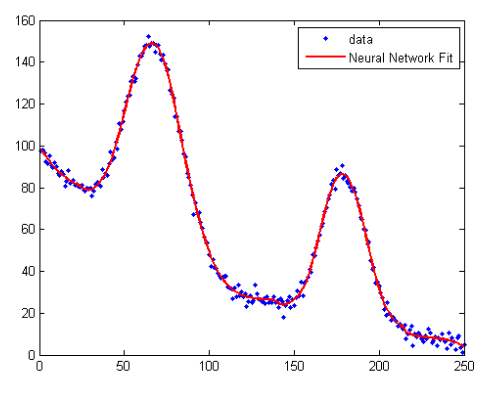
\includegraphics[width=0.9 \textwidth, keepaspectratio]{images/nn}
\end{frame}

\section{Машина опорных векторов}

\begin{frame}{Оптимальная разделяющая гиперплоскость}
	Линейно разделимая выборка:\\
	$\begin{cases}
		{\frac{1}{2} \Vert \mathbf{w} \Vert^2 \rightarrow \min\limits_{\mathbf{w}}}\\
		M_i(\mathbf{w}, w_0) \geq 1   \qquad i = 1, \dots, l
	\end{cases}$\\
	\pause
	\bigbreak
	Линейно неразделимая выборка -- надо ослабить имеющиеся условия.\\
	$\begin{cases}
		{\frac{1}{2}\Vert \mathbf{w} \Vert^2 + \textcolor{orange}{C \sum\limits_{i=1}^l \xi_i} \rightarrow \min\limits_{\mathbf{w}, \xi}}\\
		M_i(\mathbf{w}, w_0) \geq 1 - \textcolor{orange}{\xi_i} \qquad i = 1, \dots, l\\
		\textcolor{orange}{\xi_i \geq 0} \qquad i = 1, \dots, l
	\end{cases}$\\
\end{frame}

\begin{frame}{Двойственная задача SVM}
	Решение исходной задачи выражается через решение двойственной:\\
	$\begin{cases}
	\mathbf{w} = \sum\limits_{i = 1}^l \alpha_iy_i\mathbf{x_i}\\
	w_0 = \langle \mathbf{w}, \mathbf{x_i} \rangle - y_i
	\end{cases}$\\
	\bigbreak
	\pause
	$a(\mathbf{x}) = \sign(\sum\limits_{i=1}^l \alpha_iy_i \langle \mathbf{x_i}, \mathbf{x} \rangle - w_0)$
\end{frame}

\section{Как использовать для задачи регрессии?}

\begin{frame}{SVR}
  \alert{Идея}: Не считать за ошибку отклонение целевой функции меньше, чем на $\varepsilon$.
  \bigbreak
  \pause
  $\begin{cases}
		{\frac{1}{2}\Vert \mathbf{w} \Vert^2 + \textcolor{orange}{C \sum\limits_{i=1}^l (\xi_i + \hat{\xi_i}) } \rightarrow \min\limits_{\mathbf{w}, \xi}}\\
		y_i - \varepsilon - \textcolor{orange}{\xi_i} \leq \langle \mathbf{w}, \mathbf{x_i} - w_0 \rangle \leq y_i + \varepsilon + \textcolor{orange}{\xi_i} \qquad i = 1, \dots, l\\
		\textcolor{orange}{\xi_i, \hat{\xi_i} \geq 0} \qquad i = 1, \dots, l
	\end{cases}$\\
	\bigbreak
  \pause
  $a(\mathbf{x}) = \sum\limits_{i=1}^l (\alpha_i - \hat{\alpha_i}) \langle \mathbf{x_i}, \mathbf{x} \rangle - w_0$
\end{frame}

\begin{frame}{Пример}
  \centering
  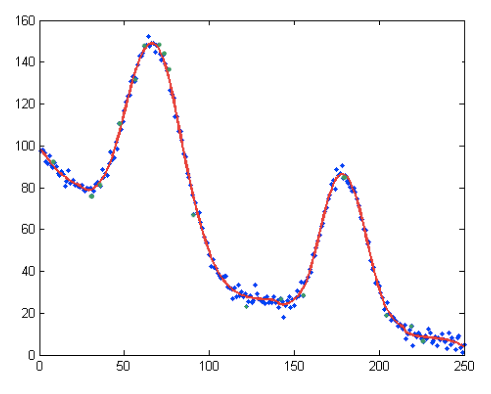
\includegraphics[width=0.9 \textwidth, keepaspectratio]{images/svr1}
\end{frame}

\begin{frame}[standout]
  Вопросы?
\end{frame}

\appendix

\begin{frame}\frametitle{На следующей лекции}
	\begin{itemize}
    	\item[--] Voting
    	\item[--] Bootstrap
    	\item[--] Bagging
    	\item[--] Boosting
    	\item[--] Adaboost
    	\item[--] Bagboo
    	\item[--] Stacking
	\end{itemize}
\end{frame}

\end{document}

\end{document}